\documentclass[conference]{IEEEtran}
%\renewcommand{\thesubsection}{\thesection.\alph{subsection}}

%\addtolength{\oddsidemargin}{-.875in}
%\addtolength{\evensidemargin}{-.875in}
%\addtolength{\textwidth}{1.75in}
%\addtolength{\topmargin}{-.875in}
%\addtolength{\textheight}{1.75in}
	
\usepackage{bm}
\usepackage{amsmath}
\usepackage{amssymb}
\usepackage{tikz}
\usetikzlibrary{automata,positioning}
\usepackage{url}
\usepackage{float}
\usepackage{setspace}
\usepackage{filecontents,lipsum}
\usepackage[noadjust]{cite}
\usepackage{listings}


\begin{document}
%\raggedright
%\doublespacing

\title{A Survey on Machine Learning: Code Smells and Antipatterns}
\author{Rodger Byrd\\rbyrd2@uccs.edu}

\maketitle

\section{Abstract}
Recently, machine learning methods have been applied to detect and correct code smells, but this is a new field and it is not mature. This paper surveys the current scientific research to review the latest information related to machine learning and code smells. An overview of code smells and antipatterns and machine learning is documented. The survey results are organized by topic and cover the current performance, detection methods, improvements to detection methods, using machine learning to correct identified smells, calssifying code smells, and using machine learing to make predictions about source code. 

\section{Introduction}
Overviews of current research on code smells are covered in \textit{A Survey on software smells} \cite{sharma_survey_2018}, \textit{A systematic literature review: Refactoring for disclosing code smells in object oriented software}\cite{singh_systematic_2018}m and \textit{Smells in software test code: A survey of knowledge in industry and
academia}\cite{garousi_smells_2018}. 
Code smell research is a growing field\cite{kokol_code_2018} as demonstrated by the increase in publishing in figure \ref{fig:smellresearch}.
\begin{figure*}[!ht]
  \centerline{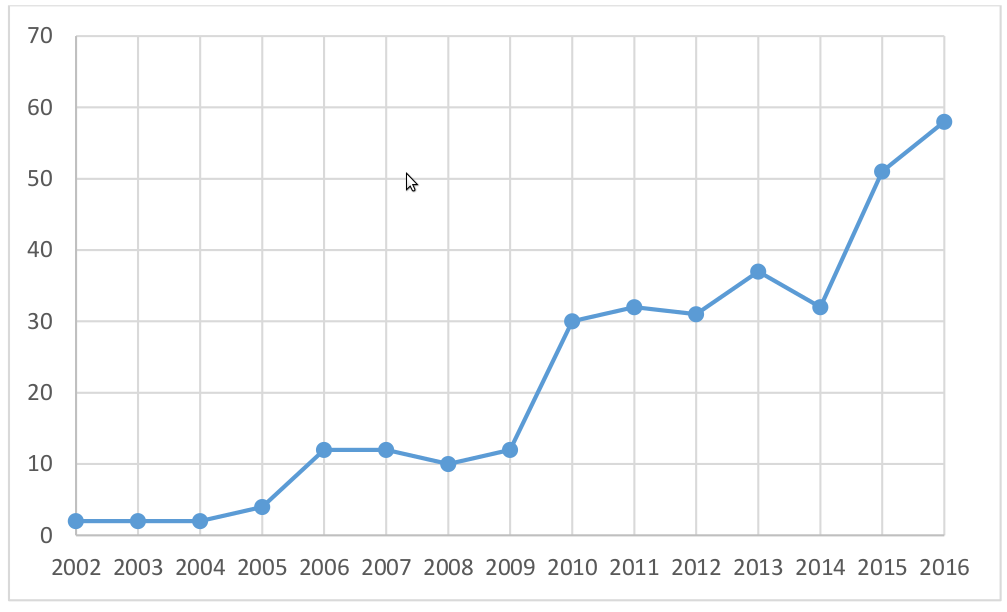
\includegraphics[width=\textwidth]{Dynamicsofcodesmellresearch.png}}
  %\centerline{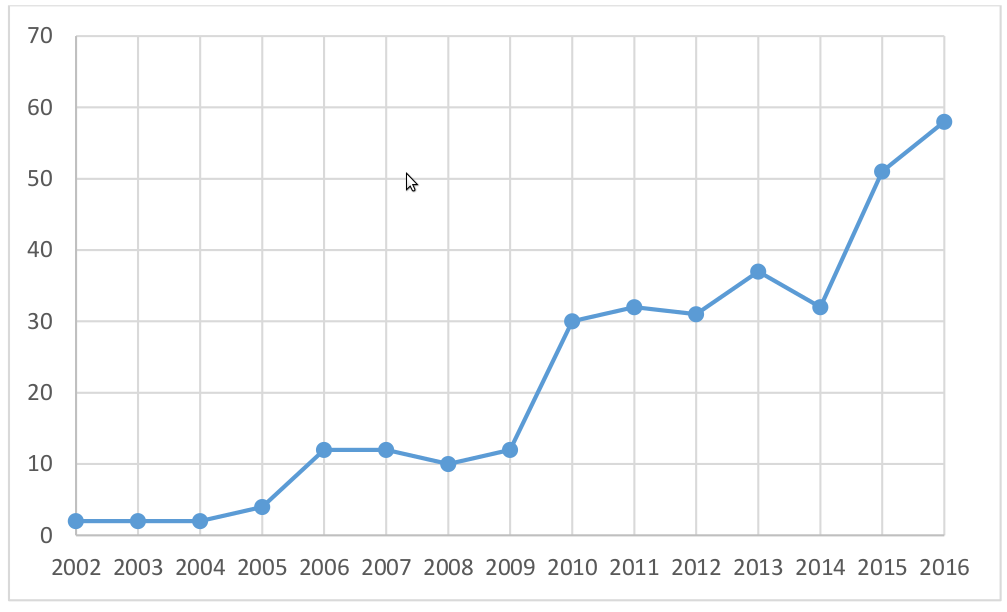
\includegraphics[width=\textwidth]{Dynamicsofcodesmellresearch.png}}
  \caption{Code smell research literature production from 2002 to 2016\cite{kokol_code_2018}}
  \label{fig:smellresearch}
\end{figure*} 
For a survey of ML and code smell detection from 2000-2017, Azeem et al. presented a systematic literature review\cite{azeem_machine_2019}. At the time, they only had 15 related papers to review. Haque et al.\cite{haque_causes_2018} performed a survey on the causes, impacts, and detection approaches of code smells but machine learning was not addressed in detail. This paper focuses exclusively on research related to code smells and machine learning.
How many papers included in this survey?
%read this later
This area of study, which is the intersection of machine learning and code smells is a rapidly growing field. 

There are five types of automated code smell detection\cite{lafi_code_2019}, they are:
\begin{enumerate}
\item Metrics based smell detection
\item Rules/heuristic-based smell detection
\item History based smell detection
\item Optimization based smell detection
\item Machine Learning based smell detection
\end{enumerate}
There are also many different tools\cite{walter_code_2018} that can be used for autometed smell detection.
Defecienies in automated tools include false-positives and lack of context, limited detection fupport for known smells, and inconsisten smell detection definitions and detectino methods\cite{sharma_detecting_2018}.
This paper will focus on the fifth type of smell detection which is machine learning.

\subsection{Code Smells and Antipatterns}
What's interesting about anti-patterns is that they have a very human aspect to them. 
They overlap the way humans think with the way code is written. 
They connect common ways of human misunderstanding to software development. 
Personally, I think most developers expect code to work as they understand it to. 
They don't spend a lot of time thinking about how code will work in ways they don't expect.
It is in the nature of most engineers to see things in mathematical/binary ways and ignore the human aspects to what they are working on.
Example boeing 737 max.
Code developers expected pilots to respond with typical emergency procedure, but when the errors occurred they pilots were overwhelmed by the amount of feedback they recieved in the cockpit (need reference).
Code smells are similar to antipatterns, but code smells may not always be bad.
Code smells can alsobe referred to as Atoms of Confusion \cite{gopstein_understanding_2017}, when referring to the smallest methods of definable smells, and nano patterrns, which are very small anti-patterns, around the size of a single method. 
An example of confusing code is shown below in in \ref{pattern1}.
Some developers will expect the output to be 25 and some will be 13 because they don't understand intuitively how the macro function works (the correct answer is 13).

\begin{lstlisting}[language=C,frame=single,caption=Example Atom of Confusion,label=pattern1]
#DEFINE M 2+3

int main() {
  int x=5, y;
  y= x * M;
  cout << y << endl;
  return 0;
}
\end{lstlisting}

Kent Beck coined the term ``code smell'' \cite{fowler_refactoring:_2018} and defined as ``certain structures in the code that suggest (sometimes they scream for) the possibility of refactoring''. They are also sometimes referred to as architecture smells.
Some common examples of code smells are as follows:
\paragraph{Large Class - Bloaters} methods and classes that have grown so large they become unsustainable, and usually accumulate over time.
\paragraph{Lazy Class} methods and classes so small they are pointless or useless.
\paragraph{Object-Oriented Abusers} misuse of object-oriented programming principles
\paragraph{Change Preventers} where multiple places in code need to be updated for a single change made somewhere else.
\paragraph{Dispensables} pointless or useless code.
\paragraph{Duplicate} code that is copy and pasted in multiple places in the code base.
\paragraph{Couplers} excessive coupling between classes.

The term antipattern was coined by Andrew Koenig \cite{koenig_patterns_1998}. 
It is defined as a commonly reinvented bad solution to a problem.
Some common examples of antipatterns are as follows:
\paragraph{Singleton Overuse} Overuse of singletons as they violate information hiding
\paragraph{Functional Decomposition} functional methods are remnants of procedural languages and conflict wiht object-oriented practices
\paragraph{Poltergeist} short-lived, limited functionality object used to perform initialization or invoke methods in another class.
\paragraph{Spaghetti} very long methods and classes with many lines of code.
\paragraph{Blob} a class with lots of attributes and methods, which can be unrelated.
\paragraph{Copy-Paste} code copied multiple times in the code base.
\paragraph{Lava Flow} Ancient code which can't be modified for fear of introducing errors.

Some papers use the terms antipatterns and code smells interchangeably\cite{singh_systematic_2018}. 
For the purposes of this paper, smells are precursors to anti-patterns. 
A code smell signals that code should be refactored and is an indicator of problem, whereas an antipattern is a definitive problem. 
The existance of code smells and antipatterns implies that there are going to be problems with software sustainment and imply there are issues with the design.


\subsection{Machine Learning}
Machine learning is defined as computers learning to solve problems without being explicitly programmed, although they are ``trained''\cite{bishop_pattern_2006}. 
Arthur Samuel coined the term Machine Learning in 1959\cite{samuel_studies_1988}.
Machine learning is a subset of artificial intelligence. 
It uses algorithms and statistical models to execute a task without explicitly being programmed.
Machine learning is used in a wide variety of applications such as email spam filtering, search engines, video surveillance, and image curation.

There are many types of learning algorithms, such as: unsupervised learning, supervised learning, reinforcement learning, self learning, feature learning, sparse dictionary learning, anomoly detection, and association rules.

Models used for machine learning include: Artificial Neural networks, decision trees, support vector machines, bayesian networks and genetic algorithms.

Machine learning techniques have been used for many different aspects of software engineering\cite{fontana_code_2017}. These include Design Pattern Detection, Code Smell Detection, Bug Prediction, and Recommending Systems among others.

Training

Training dataset vs test dataset

\section{Results}
Tian et al.\cite{tian_how_2019} and Tahir et al.\cite{tahir_can_2018} performed surveys on stack overflow related to how developers discuss code smells and antipatterns. In \cite{tian_how_2019} they found that developers have difficulty detecting and refactoring code smells due to the lack of available tools and difficulty quantifying the cost.

Variations in how the algorithms are trained, ie developer survey, evolutionary code changes
\subsection{Topic Maps}

A large topic map of antipatterns and code smells is included below in figure \ref{fig:TM}.
Machine learning is emphasized with a red circle. 
Figure \ref{fig:ML} focuses on the area of intersection between code smells and machine learning.
\begin{figure*}[ht]
  \centerline{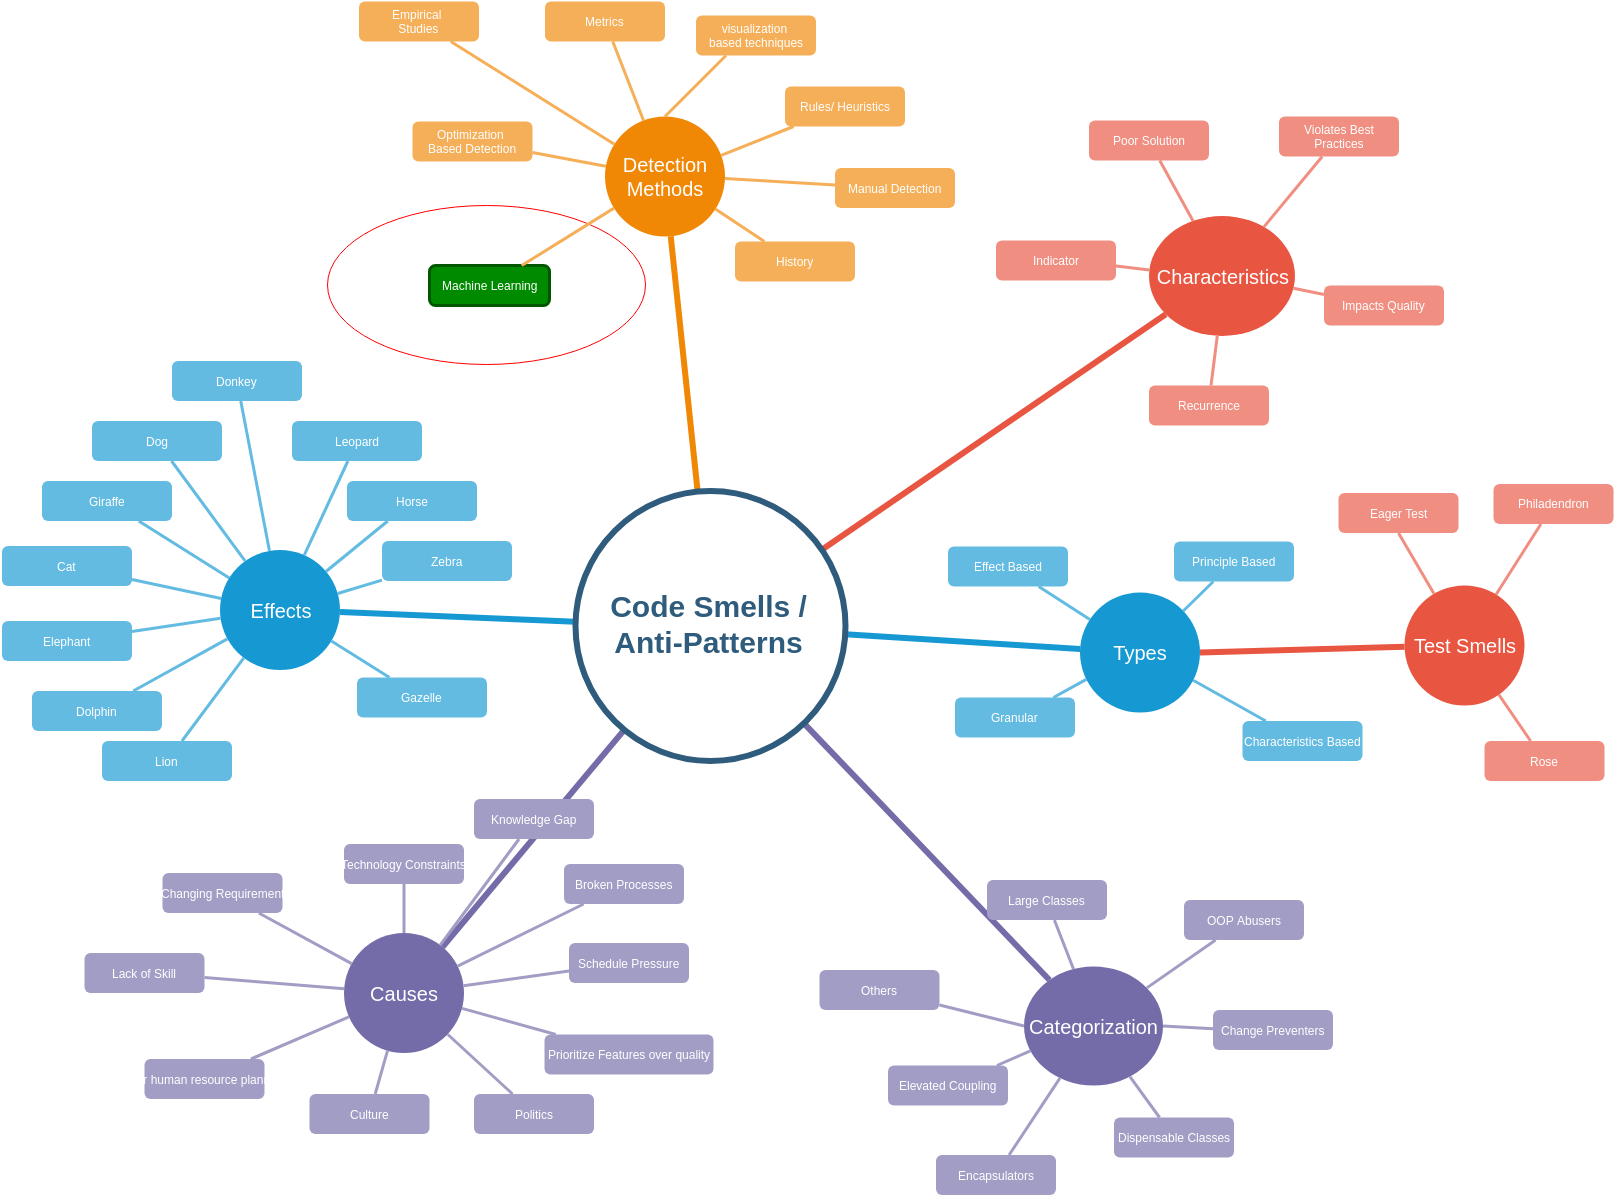
\includegraphics[width=\linewidth]{AntiPattern-TopicMap.png}}
  \caption{High level topic map on code smells and antipatterns}
  \label{fig:TM}
\end{figure*} 

\begin{figure*}[!ht]
  \centerline{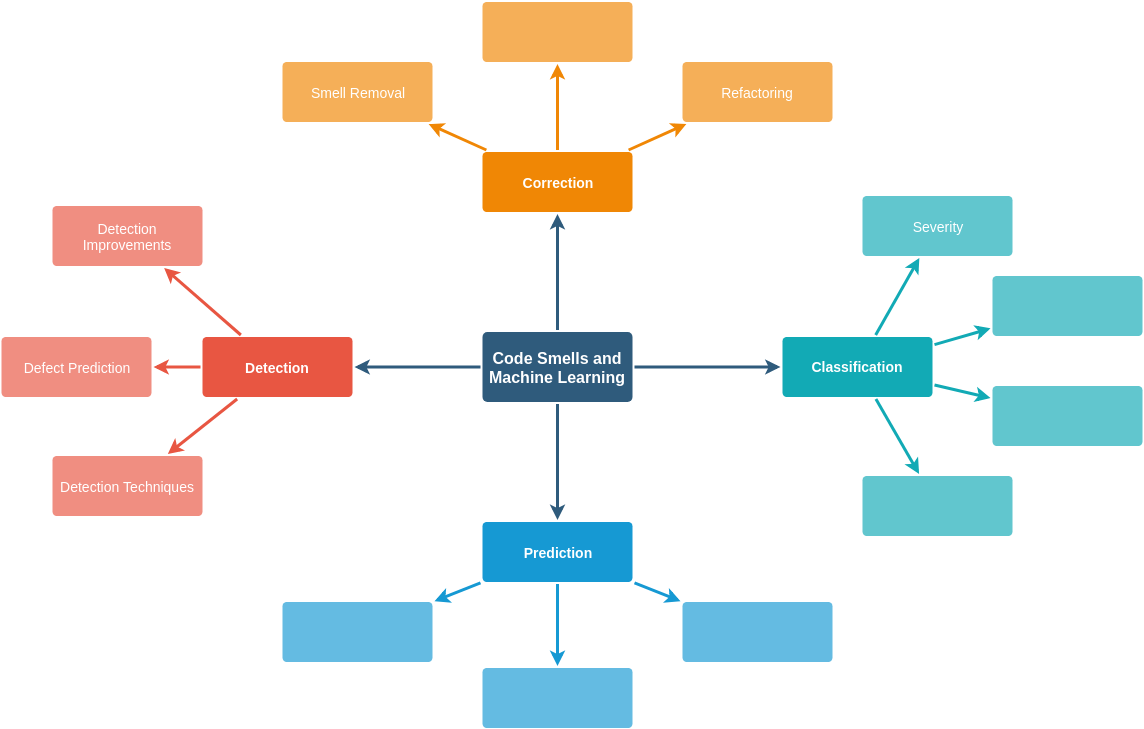
\includegraphics[width=\textwidth]{ML-codesmells.png}}
  %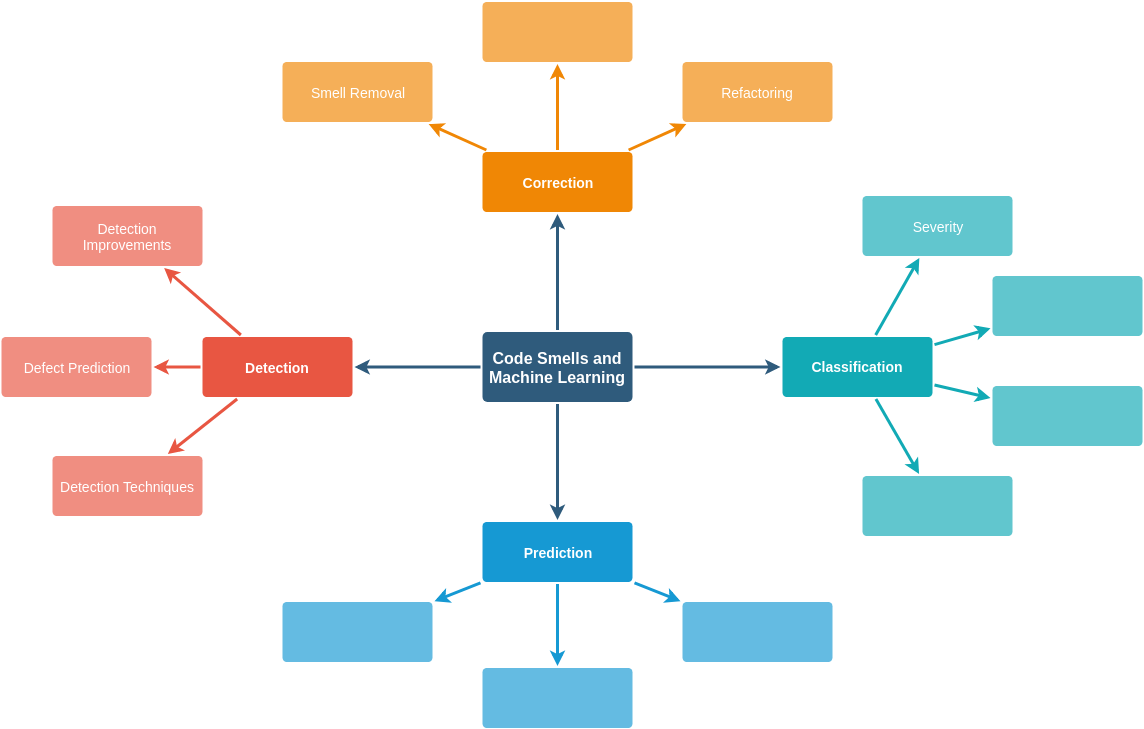
\includegraphics[width=\columnwidth]{ML-codesmells.png}
  \caption{Detail of topic map on machine learning related to code smells and antipatterns}
  \label{fig:ML}
\end{figure*} 

Include chart based on source of papers?

\subsection{Machine Learning Code Smell Detection Performance}
There are somewhat mixed results as far as the perfomance of machine learning algorithms with respect to code smell detection\cite{nucci_detecting_2018}.
In a comparison of the 32 different machine learning algorithms\cite{arcelli_fontana_comparing_2016} it was determined that the J48 and Random Forest algorithms have the best performance detecting code smells and the support vector machines had the worst performance. They also showed the algorithms had greater than 96\% accuracy and only required 100 training examples to get above 95\%.

The performance of machine learning code smell detection techniques needs to be compared to heuristic methods to determine whether it has better performance. Heruistic methods use detection rules based on software metrics. (Pecorelli et al.) showed\cite{pecorelli_comparing_2019} that their Naive Bayesian machine learning code smell detection algorithm performed at the same level or below the DECOR heuristic method. 
It can't be said for certian that all machine learning code smell detection will perform at that level as it may be due to the datasets used for training or testing.

\subsection{Code Smell Detection}
One of the larger experiments on machine learning for code smell detection was done by Fontana et al.\cite{arcelli_fontana_comparing_2016}. In this study they used 16 different machine learning algorithms on four code smells (Data Class, Large Class, Feature Envy, Long Method). It included 74 software systems and 1986 manually validated code smell samples. Many other studies use the code smell sampls to perform other research and validate this research. 
In\cite{arcelli_fontana_comparing_2016} they rank the 10 best algorithms and the top two have a large effect size meaining they had a large advantage over the remaining algorithms.
The top 10 algorithms are as follows:
\begin{enumerate}
\item B-J48 Pruned
\item Random Forest
\item B-JRip
\item B-J48 Unpruned
\item B-Random Forest
\item J48 Pruned
\item J48 Unpruned
\item JRip
\item B-J48 Reduced Error Pruning
\item J48 Reduced Error Pruning
\end{enumerate}
As shown above there are many Machine learning algorithms that can be used to detect code smells.\cite{reshi_investigating_2019}\cite{karaduzovic-hadziabdic_comparison_2018}\cite{reshi_predicting_2018}\cite{nucci_detecting_2018}\cite{karaduzovic-hadziabdic_comparison_2018}. In\cite{reshi_investigating_2019}\cite{reshi_predicting_2018} (Reshi and Singh) showed that those algorithms could be used to identify code smells implying that it could be used for preventative maintainence and to document defects or their absence in software. 
They performed the assessment on the open source Eclipse software so their work could be verifiable. Others have created novel algorithms\cite{kaur_sp-j48:_2019} like a hybrid J48 algorithm with optimization.
Other papers refer to code smells as ``Evolvability Defects''\cite{tsuda_machine_2018} but use similar methodologies such as training machine learning algorithms to detect them. In\cite{tsuda_machine_2018}, they refer to code smells as evolvability defects and antipatterns as functional defects.

\paragraph{Vulnerability Detection}
In a slightly different field but related effort, Machine learning was used to look for software vulnerabilities\cite{chernis_machine_2018}. In this research, they used machine learning with code metrics ``trivila features'' as the training dataset. These included properties like character count, entropy, max nesting depth, if-complexity and other features. It did not result in good vulnerabilty detection results.

\paragraph{Mobile Applications}
Code smells in mobile applications could lead to poor performance. Algorithms have been developed\cite{rubin_sniffing_2019}\cite{ibrahim_reducing_2018} to generate detection rules for Andriod applications. In\cite{ibrahim_reducing_2018}, algorithms have been designed to detect and refactor code semlls for mobile applications.

\paragraph{Techniques and Tools}
Tian et al.\cite{tian_how_2019} performed a survey on stack overflow related to how developers discuss code smells and antipatterns. 
They found that developers have difficulty detecting and refactoring code smells due to the lack of available tools and difficulty quantifying the cost.
Test tools for performance recognizing design smells using iPlasma with the J48 Decision Tree algorithm\cite{singh_systematic_2018} against open source software.

WekaNose is a code smell detection machine learning tool\cite{azadi_poster:_2018}. It has many of the same challengees of any machine learing algorithm that is used. It is dependent on code smell input definitions and characterization feedback on the likelihood of smell instances. 

\paragraph{Deep Learning - Neural Networks} The biggest challenge for deep learning based code smell detection\cite{liu_deep_2019} is that it requires larger training datasets than typical machine learning algorithms. In \cite{liu_deep_2019} Liu et al. showed that an automated approach for building training datasets was possible and that Deep Learning could be used to detect code smells.
In a related area, Ban et al. showed that a deep learning model could be used to identify potential vulnerabilities\cite{ban_performance_2019}, but had poor performance when facing corss-project vulnerability detection.
Liu et al. focues soley on the ``feature envy'' code smell and used deep learning to identify it in code. They also proposed automation to create their training dataset.

Other research\cite{fakhoury_keep_2018},where they refer to code smells as ``linguistic antipatterns'', has shown that deep learning did not outperform typical machine learning algorithms. In\cite{fakhoury_keep_2018}, they showed that correctly tuned, traditional machine learning classifiers can outperform deep learning for smell detection. Hardware constraints such as memory requirements resulted in much lower performance for the deep learning model against all metrics that were measured. 

\paragraph{Novel Approaches to Training Datasets}
Machine learing algorithms need to have a training dataset. One novel approach for that is to use the same codebase over time and use the deltas in code as an evolutionary training dataset\cite{wang_using_2018}. The assumptions for this are that the refactoring that happens over time will correct code smells and the algorithm can train on that dataset. In\cite{wang_using_2018} Wang et al. showed that they could identify code smells in open source datasets based on this model.
This evolutionary approach is contrary to the idea of software entropy\cite{gupta_software_2018}, which proposes that code will grow more disorderly over time, not less disorderly. The evolutionary approach may not produce consistent results for all code bases.

\paragraph{Detection on Web Services}
It is possible to predict the occurence of web-service antipatterns using source code metrics and machine learning\cite{kumar_empirical_2018}. In their test Kumar and Sureka demonstrate that Random Forest was the highest performing algorithm.

\subsection{Code Smell Detection Improvements}
Sharma et al.\cite{sharma_feasibility_2019} look at the feasability of using Transfer-learning to improve the performance of machine learing algorithms when detecting code smells. This opens the opportunity to use transfer learning to do code smell detection on programming languages where smell dection tools are not yet available.
Using machine learning code smell detection has shown that code smells are a strong predictor of class change proneness\cite{pritam_assessment_2019} with greater than 70\% probability. Software change proneness is related to its quality and sustainability.
Foidl and Felderer have proposed\cite{foidl_risk-based_2019} a risk-based approach to weight the input data quality of the machine learning algorithm with the impact of the ``badness'' of the identified code smell. 
This method could help to optimize and prioritize software maintainence efforts for large scale sustainment projects.
Barbez et al. propose\cite{barbez_machine-learning_2019} an ensemble method based deep learning algorithm for anti pattern detection which had a precision of 48\% vs the heuristic DECOR algorithm which is 35\%. Ensemble learning combines the predictions from multiple nerual

\subsection{Code Smell Correction}

\paragraph{Refactoring} It has been shown that machine learning can be used to automatically fix or propose patches for software\cite{xiong_learning_2018}. For if-statement repair Xiong et al. showed that they could use machine learning to predict code repair with 43.5\% precision.

\paragraph{Smell Removal}

\subsection{Code Smell Classification}

\paragraph{Severity} Most code smells are treated with equal severity in the works cited in this paper. Fontan and Zanoni\cite{fontana_code_2017} create a code smell severity classification using machine learning. They classify four code smells, Data Class, God Class, Feature Envy, and Long Method on a scale of 0-3 ranging from no smell to severe smell. In this experiment, they followed many of the same methods as other studies, but included a severity aspect.


\subsection{Code Smell Predictions}
Machine learning has been used to detect code smells and link those findings to bug predictions\cite{ubayawardana_bug_2018} using Naive Bayesian, Random Forest and Logistic Regression algorithms.
There are also related studies on defect prediction and software reliability prediction.
For a survey on the current stat of software defect prediciton\cite{li_progress_2018}. Li et al. have done a thorough survey including publicly available datasets and machine learning.
Additionally, sofware reliability can be predicting using machine learning techniques\cite{kulamala_predicting_2018}.

\subsection{Training Datasets}
refer to detection datasets paragraph and consolidate
%wish I had tracked these as I read through the papers, may need to re-review
% add table of datasets
In\cite{li_progress_2018}, they document many publicly available datasets for software defect prediction. This is important to compare the results of research.
A common public dataset used in many of the papers is from \cite{fontana_code_2017}. It is used in \cite{karaduzovic-hadziabdic_comparison_2018} among others.
Not all training material is equal\cite{fakhoury_keep_2018}, and for some problems like bug prediction there are abundant datasets, but other problems may require significant effort to build relevant labelled datasets.

\section{Discussion}
Most confusiong is in training datasets and identifying code smells because they can be subjectively interpreted.
Addiitionally it isnt' enought to just use expert advice/knowledge unless it has ben experimentally shown to be correct code smells. 
There must be a way to mathematically demonstrate or by experimentation that particular code patterns cause problems.
The big challenge in this field seems to be the best way to identify code smells and how training datasets are labelled and created.

The code smells and antipatterns need to be understood and identified.
Once code smell taxonomies are standardized and identified developers can change their best practices.
The best practices should be created in such a way that the typical misunderstandings of the developer can be avoided.

All the aforementioned software patterns can cause confusion to the reader of the code. Developers spend more time reading than writing (citation?) code. If thesee smells and antipatterns can be detected and corrected, it will lead to more sustainable, more stable code with less time spent by the developer so less cost as well.
Manual analysis would take so much time it is completely impractical from a cost perspecitve.
%\paragraph{Who is the Main Character}

And is what is interesting about it their human nature which leads them to confusion?
I would guess tha most developers think that a compiler is well-defined and bugs in code must be due to lack of understanding not code structure that is good at confusing human nature.

%\paragraph{What Sensory Details Will Make the Story Seem Real}
Real world examples of the problem
Temp Az, person hit by self driving car\cite{noauthor_how_nodate}

\section{Conclusion}
The problem is people don't realize they are implementing anti-patterns at the time they are writing code.
The interesting things about it are how do we find them. 
How do we detect them, and what is the fix when we identify the problem.

Because we know that the anti-patterns cause confusion in the developer, they create risk because they create unstable code. 
This is risk for the owner of the software and the customer of the developer who uses code
Machine learning algorithms have been clearly shown to be able to detect code smells, but there is no current standard approach. 
Performance varies due to different algorithms, and different training dataset approaches. 
J48 and Random Forest algorithms come up often as having the best performance detecting code smells.
Beyond the specific algorithms, the training approaches and datasets make a large difference in the performance of the algorithms. 
There are typical approaches such as surveying developers and more interesing approaches such as evolutionary approache to look at the differences in refactored code.
This points to the fact that exactly how to identify code smells and consensus on what they are speficically in code are not well defined. Multiple studies showed similar performance to the other (non-machine learning models).

These papers reference above varied widely in the number of code smells they searched for, which algorithms they used, and how they came up with trainin datasets.
Software sustainment and assurance is one of the most expensive parts of the software lifecycle\cite{li_progress_2018} and this can have a direct impact on lowering that effort and cost.


The files for this latex document are in the github repository located at \path{https://github.com/rodger79/CS6000}

%\nocite{*}

%\clearpage
\bibliographystyle{IEEEtran}
\bibliography{references}


\end{document}